\section{Off-peak Results}
\seclabel{off_peak_results}

The off-peak intervals of 54 LAT-detected pulsars have
been evaluated by \citet{ackermann_2011a_fermi-lat-search} using 16 months of sky survey observations.  
This led to the discovery of PWN-like emission
in the off-peak interval of PSR J1023$-$5746, coincident with HESS
J1023$-$575, and identification of 5 pulsars that appear to have near 100\%
duty cycles.  Our results, summarized in Table \ref{tbl-off_peak_table},
extend the analysis to 116 pulsars over 3 years of data.  
Sample off-peak spectra are shown in Figure \ref{off_peak_seds}.
Using the procedures outlined in \secref{peak_definition}
and \secref{off_peak_analysis}, we have identified 34 pulsars that
have significant emission ($TS\geq25$) in their off-peak intervals.
We classify the likely nature of the emission as follows.

If the emission has $TS_{\rm cut}\geq9$, we consider the emission to be
either magnetospheric (`M') or possibly magnetospheric (`M*').
As was discussed in \secref{off_peak_analysis}, 
we flag the emission as `M*' if the source is formally spatially extended
($TS_{\rm ext}>16$) or if the source is not robust against varying
the diffuse emission models ($\tsaltdiff<25$). 
On consideration of the angular extent of the PSF of the LAT and inaccuracies in the Galactic diffuse
emission model, we caution against considering the `M*' sources to be definitively classified.
If the source is significantly cutoff, not
significantly extended, and is significant when varying the alternative diffuse models,
we classify the emission as `M'.


On the other hand, if the
emission has $TS_{\rm ext}\geq16$, and does not suffer from confusion as
discussed at the end of \secref{off_peak_analysis}, and/or has a hard
photon index, we say it is likely
to originate in the pulsar wind and identify these sources as type `W'.
The remaining sources with off-peak emission not satisfying any of the
previous criteria are identified as type `U' to indicate that the nature
of the emission is unidentified and we do not speculate about its origin.


We identify 9 type `M' sources,
significantly expanding the number of pulsars that perhaps have detectable magnetospheric emission across all rotational phases. 
One caution is that many of these `M' pulsars, especially the young objects, are in regions of particularly bright diffuse gamma-ray
emission, where small fractional uncertainties in the level of diffuse emission can account for much of the apparent unpulsed emission. 
However, if established as true magnetospheric components, these will be important test cases for
pulsar emission models. In addition, we identify ten
`M*'-type regions.
For type `M' and `M*' sources, we present the best-fit spectral parameters using
a point source at the pulsar's position with a PLEC1 spectral model in
%columns 6, 7, and 8 of
Table \ref{tbl-off_peak_table}.  For all other
sources (except the Crab Nebula described in Sec. \ref{off_peak_analysis}), 
we present the spectral results using a power-law spectral
model and the best-fit spatial representation.


Additionally, we identified four off-peak emissions consistent with a PWN
hypothesis, one of them being a new detection at GeV energies (PSR J0205+6449).
Only one of these four, the previously identified Vela$-$X PWN \citep{abdo_2010c_fermi-large}, is spatially extended for the LAT.
Similarly, we detect six type `U' regions. Three of these are formally 
spatially extended
but because of the spatial systematics 
we assume point-like emission for the spectral analysis.

We mention that for a few sources, the spectral analysis
performed here is in disagreement with the analysis presented in
\citet{ackermann_2011a_fermi-lat-search}. For soft and faint sources
(including J1044$-$5737 and J1809$-$2332), the spectral discrepancy is
mainly caused by our use of a newer Galactic diffuse model. At lower
energies, small changes in the diffuse model can have a significant
impact on the analysis of a region.  For bright magnetospheric sources
(including J0633+1746 and J2021+4026), the spectral discrepancy is mainly
due to using different phase ranges (see Sec.~\ref{peak_definition}).


\figref{off_peak_luminosity_vs_edot} shows that only
a small fraction of the spindown power goes into 
the gamma-ray emission from LAT-detected PWNe.
Similarly, 
Figure~\ref{P0_sqEDOTD2} shows that the LAT only detects
PWNe from the youngest pulsars with the highest spindown power.
GeV emission from the Crab Nebula is highly time variable (\secref{off_peak_analysis}).  
Indeed, we find
$TS_{\rm var}=373$ for the Crab Nebula; however
no other source demonstrated flux variability (all have $16 <TS_{\rm var} <65)$.  
Other GeV PWNe may be variable, but the combination of lower fluxes
and less-extreme variations limits our ability identify them as such.


The off-peak results for several interesting sources are
presented in Appendix~\ref{App-off_peak_individual_source_discussion}.
The complete off-peak search results can be found in the accompanying
auxiliary information described in Appendix \ref{off_peak_auxiliary}.
For regions where we find $TS<25$, the auxiliary information contains
upper limits computed for both a power-law spectral model and a
PLEC1 model with $E_{\rm cut}=3$ GeV and $\Gamma=1.7$.  The auxiliary
information also contains $TS_{\rm var}$ for each off-peak interval.



\begin{deluxetable}{ll*{8}c}
\tablecolumns{8}
\tablewidth{0pt}
\tabletypesize{\scriptsize}
\tablecaption{Off-Peak Spatial and Spectral Results
\tablabel{tbl-off_peak_table}
}
\tablehead{\colhead{PSR} & \colhead{Type} & \colhead{$\tspoint$} & \colhead{$\tsext$} & \colhead{$\tscutoff$} & \colhead{$\tsaltdiff$} & \colhead{Energy Flux} & \colhead{$\Gamma$} & \colhead{$\Ecutoff$}\\ \colhead{ } & \colhead{ } & \colhead{ } & \colhead{ } & \colhead{ } & \colhead{ } & \colhead{($10^{-11}\,\efluxunits$)} & \colhead{ } & \colhead{(GeV)}}
\startdata
\multicolumn{8}{c}{Young Pulsars} \\[3pt]
\hline
J0007+7303 & U & 71.4 & 10.8 & 0.0 &  & $1.98 \pm 0.26$ & $2.61 \pm 0.14$ &  \\
J0205+6449 & W & 33.7 & 0.5 & 0.0 &  & $1.75 \pm 0.68$ & $1.61 \pm 0.21$ &  \\
J0534+2200 & W & 5247. & 0.0 & 0.3 &  & $67.2 \pm 1.6$ & \tablenotemark{a} &  \\
J0631+1036 & U & 33.1 & 0.0 & 5.4 &  & $1.70 \pm 0.33$ & $2.38 \pm 0.14$ &  \\
J0633+1746 & M & 3666. & 2.3 & 239. & 3369. & $41.4 \pm 1.1$ & $1.37 \pm 0.09$ & $0.93 \pm 0.10$ \\
J0734$-$1559 & M* & 28.3 & 12.4 & 30.8 & 0.0 & $1.61 \pm 0.24$ & $0.01 \pm 0.08$ & $0.17 \pm 0.03$ \\
J0835$-$4510 & W & 473. & 283. & 22.8 &  & $30.3 \pm 1.2$ & \tablenotemark{b} &  \\
J0908$-$4913 & M* & 65.1 & 41.4 & 60.4 & 3.1 & $3.04 \pm 1.07$ & $0.15 \pm 0.59$ & $0.30 \pm 0.01$ \\
J1023$-$5746 & M* & 59.7 & 30.0 & 10.9 & 72.5 & $5.35 \pm 1.17$ & $0.57 \pm 0.80$ & $0.49 \pm 0.21$ \\
J1044$-$5737 & M* & 42.0 & 98.1 & 22.4 & 25.6 & $3.12 \pm 0.75$ & $0.80 \pm 0.93$ & $0.40 \pm 0.18$ \\
J1105$-$6107 & M* & 33.3 & 37.5 & 21.7 & 39.4 & $3.81 \pm 0.77$ & $0.92 \pm 0.56$ & $0.48 \pm 0.22$ \\
J1112$-$6103 & U & 65.0 & 71.1 & 0.9 &  & $5.10 \pm 0.74$ & $2.17 \pm 0.09$ &  \\
J1119$-$6127 & U & 61.3 & 1.0 & 0.9 &  & $4.11 \pm 0.63$ & $2.22 \pm 0.09$ &  \\
J1124$-$5916 & M & 95.9 & 0.0 & 18.2 & 59.4 & $2.87 \pm 0.71$ & $1.31 \pm 0.91$ & $1.43 \pm 1.42$ \\
J1410$-$6132 & U & 27.5 & 71.2 & 0.4 &  & $4.29 \pm 1.05$ & $1.90 \pm 0.15$ &  \\
J1513$-$5908 & W & 102. & 3.5 & 0.0 &  & $4.95 \pm 0.83$ & $1.78 \pm 0.12$ &  \\
J1620$-$4927 & M* & 28.9 & 0.5 & 35.2 & 0.0 & $5.25 \pm 0.96$ & $0.35 \pm 0.94$ & $0.57 \pm 0.29$ \\
J1746$-$3239 & M* & 53.3 & 34.3 & 34.2 & 0.0 & $3.65 \pm 0.59$ & $0.94 \pm 0.31$ & $0.60 \pm 0.10$ \\
J1747$-$2958 & M & 45.5 & 5.4 & 49.8 & 50.4 & $8.41 \pm 2.84$ & $0.02 \pm 0.32$ & $0.28 \pm 0.01$ \\
J1809$-$2332 & M* & 32.5 & 13.6 & 21.9 & 0.0 & $4.10 \pm 0.80$ & $0.24 \pm 0.83$ & $0.31 \pm 0.11$ \\
J1813$-$1246 & M & 62.8 & 0.0 & 9.0 & 49.7 & $6.31 \pm 1.40$ & $1.60 \pm 0.73$ & $0.99 \pm 0.95$ \\
J1836+5925 & M & 10407. & 0.0 & 365. & 10401. & $36.9 \pm 0.7$ & $1.47 \pm 0.03$ & $1.98 \pm 0.09$ \\
J1838$-$0537 & M* & 51.3 & 32.9 & 21.9 & 41.9 & $8.35 \pm 1.31$ & $1.39 \pm 0.54$ & $2.55 \pm 2.48$ \\
J2021+4026 & M & 1717. & 8.7 & 244. & 1978. & $64.0 \pm 1.4$ & $1.64 \pm 0.02$ & $1.82 \pm 0.04$ \\
J2032+4127 & U & 53.6 & 76.1 & 1.5 &  & $4.36 \pm 0.77$ & $2.07 \pm 0.12$ &  \\
J2055+2539 & M & 123. & 0.0 & 30.0 & 101. & $1.63 \pm 0.19$ & $1.05 \pm 0.28$ & $0.64 \pm 0.12$ \\
\hline\\[-5pt]
\multicolumn{8}{c}{Millisecond Pulsars} \\[3pt]
\hline
J0034$-$0534 & U & 41.0 & 0.0 & 6.0 &  & $0.82 \pm 0.16$ & $2.40 \pm 0.19$ &  \\
J0102+4839 & U & 49.7 & 0.0 & 7.4 &  & $1.29 \pm 0.20$ & $2.51 \pm 0.14$ &  \\
J0218+4232 & U & 50.1 & 0.0 & 6.8 &  & $2.13 \pm 0.33$ & $2.72 \pm 0.26$ &  \\
J0340+4130 & M* & 26.9 & 0.1 & 16.3 & 11.9 & $0.53 \pm 0.11$ & $0.02 \pm 0.22$ & $0.94 \pm 0.28$ \\
J1658$-$5324 & U & 42.3 & 0.0 & 1.9 &  & $1.69 \pm 0.29$ & $2.52 \pm 0.76$ &  \\
J2043+1711 & U & 52.5 & 0.0 & 8.8 &  & $1.46 \pm 0.27$ & $2.29 \pm 0.14$ &  \\
J2124$-$3358 & M & 129. & 0.0 & 19.8 & 118. & $1.08 \pm 0.15$ & $0.70 \pm 0.51$ & $1.21 \pm 0.49$ \\
J2302+4442 & M & 114. & 0.0 & 9.8 & 105. & $1.45 \pm 0.20$ & $1.54 \pm 0.40$ & $1.61 \pm 0.82$ \\
\enddata


\tablenotetext{a}{The spectral shape of the Crab Nebula was taken from \citet{buehler_2012a_gamma-ray-activity}.}
\tablenotetext{b}{The spectral shape of Vela$-$X was taken from \cite{grondin_2013a_vela-x-pulsar}.}

\tablecomments{Off-peak regions with a significant detection of emission.
The source classification is `M' for likely magnetospheric, 
`M*' for possibly magnetospheric but with a problematic spatial analysis or in a region with possibly poorly-modeled
Galactic diffuse emission,
`W' for likely pulsar wind, and `U' for unidentified.
The table includes the significance of the source ($TS$),  
of the source extension ($TS_{\rm ext}$), of a spectral cutoff ($TS_{\rm cut}$),
and with the alternative diffuse models ($\tsaltdiff$). 
The best-fit energy flux and photon index are computed in the energy range from 100 \mev to 316 \gev.
For sources with large $TS_{\rm cut}$, the exponential cutoff energies are presented. 
The quoted errors are statistical only. A few sources are discussed in \secref{off_peak_individual_source_discussion}.
}


\end{deluxetable}

\begin{figure}
  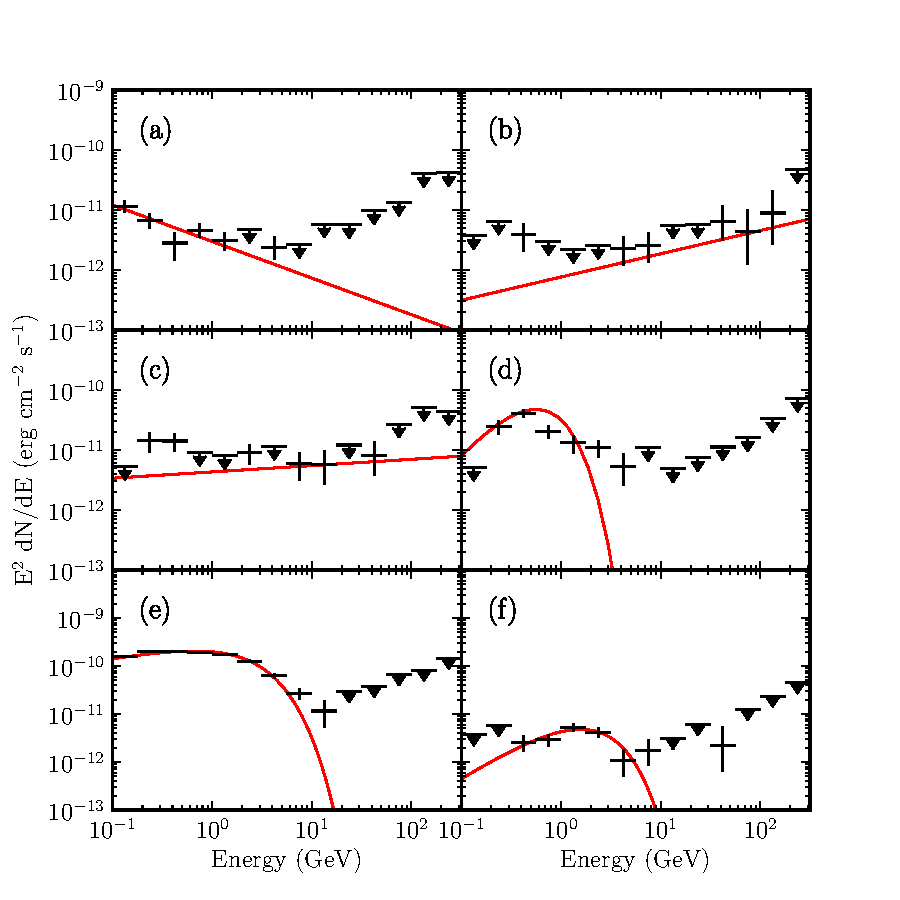
\includegraphics{chapters/offpeak/figures/off_peak_seds_color.pdf}
  \caption{Spectral energy distributions for the off-peak
  phase intervals around
  (a) PSR J0007+7303 (b) PSR J0205+6449, (c) PSR J1410$-$6132,
  (d) PSR J1747$-$2958, (e) PSR J2021+4026, and (f) PSR J2124$-$3358.
  We plot a detection in those energy bands in which the source is found with $TS\geq4$ (a $2\sigma$ detection) and report a Bayesian 95\% confidence-level upper limit otherwise.  The best-fit spectral model, using the full energy range, is also shown for comparison.
  }
  \figlabel{off_peak_seds}
\end{figure}

\begin{figure}
  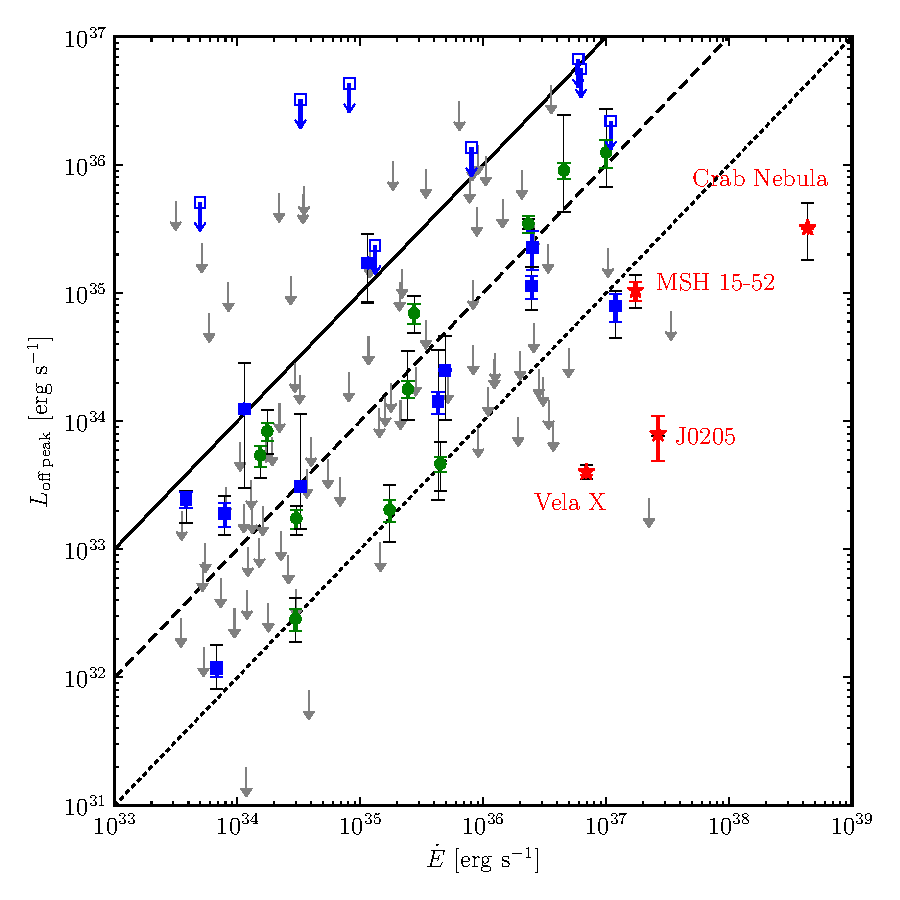
\includegraphics{chapters/offpeak/figures/off_peak_luminosity_vs_edot_color.pdf}
  \caption{The off-peak luminosity compared to the observed pulsar spindown power. 
  The luminosity is computed and plotted with the same convention as
  Figure~\ref{EDotLumG}. A luminosity upper limit is plotted
  when there is no significant off-peak emission or when there
  is only a distance upper limit.
  The
  star-shaped markers (colored red in the online version) represent
  type `W' sources, the square-shaped markers (colored blue) represent type `M' 
  and `M*' sources, 
  circular markers (colored green) represent type `U' sources,
  and the gray arrows represent non-detections.
  The filled blue square-shaped markers represent `M' and `M*' sources
  with a detected luminosity and the unfilled markers represent luminosity
  upper limits where there is only a distance upper limit.
  The solid, dashed, and dotted diagonals show 100\%, 10\%, and 1\% efficiency
  (respectively).
  }
  \figlabel{off_peak_luminosity_vs_edot}
\end{figure}
